\begin{figure}[t!]
\vspace*{-2ex}
\centering
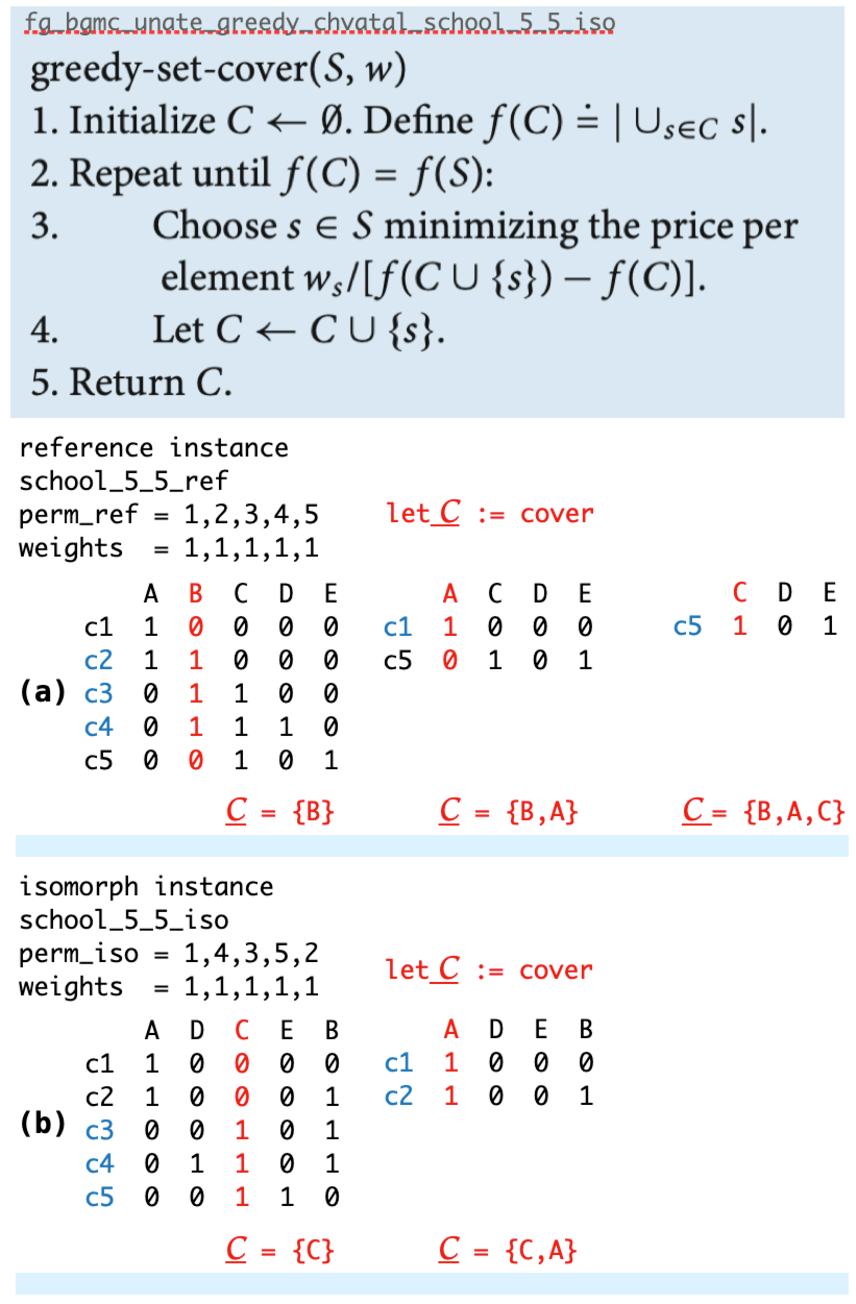
\includegraphics[width=0.45\textwidth]{_Figures/fg_bgmc_unate_greedy_chvatal_iso_school_5_5}
\caption{
The pseudo code of the greedy algorithm above is 
from~\cite{OPUS-setc-2016-Springer-Young-Greedy};
it represents the version of the Chvatal's algorithm 
in~\cite{OPUS-setc-1979-OR-Chvatal-greedy}.
The R-function that implements this algorithm is named
{\tt unate\_greedy\_chvatal\_basic} 
in Figure~\ref{fg_bgmc_unate_greedy_chvatal_stoc}a.
%
The algorithm is invoked on two instance bigraphs, represented
as two incidence matrices:
(a) the reference instance {\tt school\_5\_5\_ref}, and 
(b) the instance isomorph  {\tt school\_5\_5\_iso}.
As implied by the matrix structure, the weight of each column is 1.
For (a), the algorithm selects the 
{\it first column with minimum rate between column weight and column degree},
i.e. column B. In the next iteration, there remain only two rows to consider: s1 and s5. The first column with maximum degree is now column A. The algorithm terminates by selecting column C, returning a solution as 3 columns \{B, A, C\} and the total weight of 3.
%
For (b), the algorithm selects C as the first column with minimum rate between column weight and column degree. The next iteration is also the last. With the selection of
column A,  we get a solution as 2 columns \{C, A\} and the total weight of 2.
\vspace*{-4ex}
}
\label{fg_bgmc_unate_greedy_chvatal_iso_school_5_5}
\end{figure}
